% !TEX TS-program = XeLaTeX
% use the following command:
% all document files must be coded in UTF-8
\documentclass[portuguese]{textolivre}
% build HTML with: make4ht -e build.lua -c textolivre.cfg -x -u article "fn-in,svg,pic-align"

\journalname{Texto Livre}
\thevolume{18}
%\thenumber{1} % old template
\theyear{2025}
\receiveddate{\DTMdisplaydate{2025}{5}{7}{-1}} % YYYY MM DD
\accepteddate{\DTMdisplaydate{2025}{6}{4}{-1}}
\publisheddate{\DTMdisplaydate{2025}{9}{18}{-1}}
\corrauthor{Karla Angélica Silva do Nascimento}
\articledoi{10.1590/1983-3652.2025.59011}
%\articleid{NNNN} % if the article ID is not the last 5 numbers of its DOI, provide it using \articleid{} commmand 
% list of available sesscions in the journal: articles, dossier, reports, essays, reviews, interviews, editorial
\articlesessionname{articles}
\runningauthor{Araújo e Pereira} 
%\editorname{Leonardo Araújo} % old template
\sectioneditorname{Daniervelin Pereira}
\layouteditorname{Saula Cecília}

\title{Realidade aumentada no ensino de modelos atômicos: engajamento e motivação no ensino fundamental}
\othertitle{Augmented reality in the teaching of atomic models: engagement and motivation in primary education}
% if there is a third language title, add here:
%\othertitle{Artikelvorlage zur Einreichung beim Texto Livre Journal}

\author[1]{Karla Angélica Silva do Nascimento~\orcid{0000-0001-6103-2397}\thanks{Email: \href{mailto:karla.angelica@uece.br}{karla.angelica@uece.br}}}
\author[2]{Viviane dos Santos Marques~\orcid{0000-0003-0692-0548}\thanks{Email: \href{mailto:vsmarques124@gmail.com}{vsmarques124@gmail.com}}}
\affil[1]{Universidade Estadual do Ceará, Faculdade de Educação e Ciências Integradas do Sertão de Canindé, Programa de Pós-Graduação em Educação, Fortaleza, Ceará, Brasil.}
\affil[2]{Rede Municipal de Ensino, Meruoca, Ceará, Brasil.}

\addbibresource{article.bib}
% use biber instead of bibtex
% $ biber article

% used to create dummy text for the template file
\definecolor{dark-gray}{gray}{0.35} % color used to display dummy texts
\usepackage{lipsum}
\SetLipsumParListSurrounders{\colorlet{oldcolor}{.}\color{dark-gray}}{\color{oldcolor}}

% used here only to provide the XeLaTeX and BibTeX logos
\usepackage{hologo}

% if you use multirows in a table, include the multirow package
\usepackage{multirow}

% provides sidewaysfigure environment
\usepackage{rotating}

% CUSTOM EPIGRAPH - BEGIN 
%%% https://tex.stackexchange.com/questions/193178/specific-epigraph-style
\usepackage{epigraph}
\renewcommand\textflush{flushright}
\makeatletter
\newlength\epitextskip
\pretocmd{\@epitext}{\em}{}{}
\apptocmd{\@epitext}{\em}{}{}
\patchcmd{\epigraph}{\@epitext{#1}\\}{\@epitext{#1}\\[\epitextskip]}{}{}
\makeatother
\setlength\epigraphrule{0pt}
\setlength\epitextskip{0.5ex}
\setlength\epigraphwidth{.7\textwidth}
% CUSTOM EPIGRAPH - END

% to use IPA symbols in unicode add
%\usepackage{fontspec}
%\newfontfamily\ipafont{CMU Serif}
%\newcommand{\ipa}[1]{{\ipafont #1}}
% and in the text you may use the \ipa{...} command passing the symbols in unicode

% LANGUAGE - BEGIN
% ARABIC
% for languages that use special fonts, you must provide the typeface that will be used
% \setotherlanguage{arabic}
% \newfontfamily\arabicfont[Script=Arabic]{Amiri}
% \newfontfamily\arabicfontsf[Script=Arabic]{Amiri}
% \newfontfamily\arabicfonttt[Script=Arabic]{Amiri}
%
% in the article, to add arabic text use: \textlang{arabic}{ ... }
%
% RUSSIAN
% for russian text we also need to define fonts with support for Cyrillic script
% \usepackage{fontspec}
% \setotherlanguage{russian}
% \newfontfamily\cyrillicfont{Times New Roman}
% \newfontfamily\cyrillicfontsf{Times New Roman}[Script=Cyrillic]
% \newfontfamily\cyrillicfonttt{Times New Roman}[Script=Cyrillic]
%
% in the text use \begin{russian} ... \end{russian}
% LANGUAGE - END

% EMOJIS - BEGIN
% to use emoticons in your manuscript
% https://stackoverflow.com/questions/190145/how-to-insert-emoticons-in-latex/57076064
% using font Symbola, which has full support
% the font may be downloaded at:
% https://dn-works.com/ufas/
% add to preamble:
% \newfontfamily\Symbola{Symbola}
% in the text use:
% {\Symbola }
% EMOJIS - END

% LABEL REFERENCE TO DESCRIPTIVE LIST - BEGIN
% reference itens in a descriptive list using their labels instead of numbers
% insert the code below in the preambule:
%\makeatletter
%\let\orgdescriptionlabel\descriptionlabel
%\renewcommand*{\descriptionlabel}[1]{%
%  \let\orglabel\label
%  \let\label\@gobble
%  \phantomsection
%  \edef\@currentlabel{#1\unskip}%
%  \let\label\orglabel
%  \orgdescriptionlabel{#1}%
%}
%\makeatother
%
% in your document, use as illustraded here:
%\begin{description}
%  \item[first\label{itm1}] this is only an example;
%  % ...  add more items
%\end{description}
% LABEL REFERENCE TO DESCRIPTIVE LIST - END


% add line numbers for submission
%\usepackage{lineno}
%\linenumbers

\begin{document}
\maketitle

\begin{polyabstract}
\begin{abstract}
Este estudo teve como objetivo identificar os impactos da Realidade Aumentada no engajamento e na motivação de estudantes do 9º ano do Ensino Fundamental durante o aprendizado de modelos atômicos. Por meio de uma abordagem qualitativa, com análise de discurso, a pesquisa foi conduzida em uma escola pública utilizando o aplicativo \emph{Modelos Atômicos 3D} integrado às aulas de ciências. A interação com objetos virtuais proporcionada pela tecnologia buscou tornar conteúdos abstratos mais acessíveis e estimular o envolvimento cognitivo e emocional dos alunos. Os resultados apontaram um aumento significativo no interesse, participação e compreensão dos estudantes, além de favorecer a autonomia e o protagonismo discente. O estudo também evidenciou desafios, como a escassez de pesquisas que correlacionem diretamente o uso da Realidade Aumentada com indicadores objetivos de engajamento e motivação. Conclui-se que a integração de recursos digitais inovadores pode tornar o ensino mais interativo e significativo, ressaltando a necessidade de políticas públicas e formação docente para ampliar o acesso a essas ferramentas na educação básica.

\keywords{Realidade virtual\sep Realidade aumentada\sep Química\sep Engajamento cognitivo}
\end{abstract}

\begin{english}
\begin{abstract}
The aim of this study was to identify the impact of Augmented Reality on the engagement and motivation of 9th-grade students when learning about atomic models. Using a qualitative approach with discourse analysis, the research was conducted in a public school using the \emph{3D Atomic Models} application integrated into science lessons. The interaction with virtual objects provided by the technology sought to make abstract content more accessible and stimulate students' cognitive and emotional involvement. The results showed a significant increase in student interest, participation and understanding, as well as fostering student autonomy and protagonism. The study also highlighted challenges, such as the scarcity of research that directly correlates the use of Augmented Reality with objective indicators of engagement and motivation. The conclusion is that the integration of innovative digital resources can make teaching more interactive and meaningful, highlighting the need for public policies and teacher training to increase access to these tools in basic education.

\keywords{Virtual reality\sep Augmented reality\sep Chemistry\sep Cognitive engagement}
\end{abstract}
\end{english}
% if there is another abstract, insert it here using the same scheme
\end{polyabstract}

\section{Introdução}\label{sec-intro}
A utilização de tecnologias imersivas, como a Realidade Virtual (RV) e a Realidade Aumentada (RA), tem se mostrado uma estratégia promissora para transformar o ensino de ciências, especialmente em conteúdos abstratos como os modelos atômicos. Enquanto a RV cria ambientes digitais totalmente imersivos, a RA sobrepõe elementos virtuais ao mundo real, permitindo que os alunos interajam com conceitos complexos de forma tangível e contextualizada. Estudos recentes \cite{santos2023, tito2022} demonstram que essas ferramentas potencializam o engajamento e a motivação, alinhando-se aos princípios construtivistas ao conceder aos estudantes autonomia para explorar, manipular e refletir sobre seu próprio aprendizado.

A integração da RA no ensino de ciências da natureza tem se destacado como um recurso capaz de superar limitações metodológicas tradicionais, especialmente em temas que exigem visualização tridimensional e interação prática. Essas pesquisas também apontam que o uso de aplicativos com RA em aulas de ciências aumenta significativamente a motivação e a retenção de conteúdos, mesmo em escolas com infraestrutura limitada.

O uso da RA no ensino possibilita uma abordagem mais inclusiva e diversificada, atendendo diferentes estilos e ritmos de aprendizagem. Conforme apontam \textcite{caberoalmenara2023carga}, embora a RA possa facilitar a compreensão de conteúdos complexos ao apresentar informações de forma visual, interativa e contextualizada, seu impacto na carga cognitiva depende do \textit{design} das atividades e da familiaridade dos estudantes com a tecnologia. Essa característica é especialmente relevante para o ensino de modelos atômicos, cujo caráter abstrato frequentemente dificulta a compreensão por meio de métodos tradicionais.

Ademais, a RA promove competências digitais e cognitivas essenciais que permitem a visualização de conceitos abstratos e a interação com modelos 3D no mundo real. Assim, os alunos desenvolvem habilidades visuoespaciais e pensamento crítico por meio da manipulação de objetos virtuais em tempo real. Essas tecnologias são particularmente relevantes em contextos de educação básica, onde a abstração de conceitos científicos muitas vezes gera desinteresse e dificuldades de aprendizagem.

Entretanto, para que essas tecnologias alcancem seu potencial, é fundamental investir na formação continuada dos professores e na infraestrutura adequada das escolas, sobretudo públicas. \textcite{nascimento2016, nascimento2017} destacam que a simples disponibilização de dispositivos móveis e aplicativos não garante a efetividade pedagógica; é necessária uma integração planejada e contextualizada dessas ferramentas ao currículo escolar.

Outro aspecto está relacionado ao pouco conhecimento acerca dessas tecnologias, por exemplo: a escassez de pesquisas que correlacionem o uso de RA com indicadores específicos de engajamento -- tempo de interação, participação ativa --, motivação autônoma e a necessidade de compreender como esses recursos podem ser integrados a currículos de escolas públicas, onde limitações tecnológicas e formação docente são frequentemente críticas.

No tocante à motivação autônoma, segundo \textcite{deci2008}, está ligada diretamente à Teoria da Autodeterminação, visto que todo comportamento intencional pode ser regulado de forma autônoma ou controlada: a regulação autônoma ocorre quando o indivíduo age por vontade própria, interesse pessoal e valores internos, enquanto a regulação controlada decorre de pressões externas, recompensas ou obrigações. A autodeterminação é definida como a experiência subjetiva de autonomia, envolvendo três componentes fundamentais: lócus interno de causalidade (a percepção de que a ação parte de si mesmo), liberdade psicológica e percepção de escolha. A teoria destaca que a motivação autônoma -- que inclui a motivação intrínseca -- está associada à satisfação das necessidades de competência, autonomia e pertencimento, fatores essenciais para o engajamento, persistência e desempenho de qualidade no processo de aprendizagem. Por isso, essa Teoria é amplamente reconhecida na literatura como fundamento para compreender como a autonomia e o interesse genuíno potencializam o aprendizado, em contraste com abordagens baseadas apenas em recompensas, como a extrínseca, que depende de estímulos e controles externos para promover o engajamento do estudante.

Apesar dos avanços, ainda há carência de evidências específicas sobre como a RA influencia a motivação autônoma e o engajamento cognitivo em comparação com métodos expositivos tradicionais. Este estudo busca responder à pergunta: como a interação com modelos atômicos em RA favorece a motivação autônoma e o engajamento cognitivo de estudantes em comparação com métodos tradicionais? A resposta a essa questão é crucial para orientar políticas públicas e formação docente, especialmente em escolas públicas onde a falta de recursos tecnológicos e capacitação ainda é um obstáculo.

O objetivo desta investigação foi identificar os impactos da RA no engajamento e motivação de estudantes do 9º ano do Ensino Fundamental durante o aprendizado de modelos atômicos. A análise focou não apenas nos resultados educacionais, mas também nas percepções discentes e docentes, oferecendo insights para políticas educacionais e formação de professores.

\section{Metodologia}
A pesquisa adotou uma abordagem qualitativa que, segundo \textcite{minayo2012}, busca interpretar o universo dos sujeitos em seus contextos, valorizando a perspectiva dos participantes e a construção social da realidade. Ancorada na Análise do Discurso, que considera os contextos social, histórico e ideológico na produção de sentidos \cite{brandao2009}, investigaram-se os impactos da Realidade Aumentada no engajamento e na motivação de estudantes do 9º ano do Ensino Fundamental durante o aprendizado de modelos atômicos. O estudo foi realizado em uma escola pública, situada na região Nordeste do Brasil, onde a aplicação \emph{Modelos Atómicos 3D} (LIITEC-ULS)\footnote{Aplicativo espanhol desenvolvido pelo Laboratório de Pesquisa e Inovação Tecnológica para o Ensino de Ciências (LIITEC-ULS), uma iniciativa interdepartamental da Universidade de La Serena, localizada na cidade de Coquimbo, Chile.} foi integrada às aulas de ciências, e utilizaram-se estratégias metodológicas focadas na linguagem e nas narrativas dos participantes como elementos centrais para compreender processos subjetivos e sociais.

A coleta de dados teve como base a observação participante \cite{martins1996}, priorizando a captura de discursos espontâneos e mediados durante o uso da RA. Essas observações registraram não apenas as interações físicas dos alunos com os modelos 3D, mas também expressões verbais e diálogos coletivos que emergiam durante as atividades.

A análise seguiu os princípios da Análise do Discurso \cite{brandao2009}, integrando três dimensões: (1) o exame linguístico das transcrições, com destaque para expressões espontâneas como ``parecia que eu tocava nas moléculas" e ``isso me fez entender o que a professora explicou no quadro", que evidenciam a ressignificação dos conceitos por parte dos estudantes; (2) a investigação de como os discursos são produzidos, distribuídos e consumidos no contexto escolar, destacando diferenças nas narrativas entre alunos com maior domínio tecnológico e aqueles que enfrentaram dificuldades técnicas; e (3) a análise da relação entre os discursos e as estruturas de poder/influência na sala de aula, refletindo sobre como a inserção da RA pode ter tensionado ou transformado hierarquias tradicionais entre professores e alunos.

A comparação entre discursos de alunos, registros de observação e materiais pedagógicos utilizados (exemplo: guia de atividades do LIITEC-ULS), permitiu cruzar perspectivas individuais e coletivas. O estudo também acompanhou a turma na atividade, para capturar mudanças discursivas ao longo do tempo (exemplo: transição de narrativas de estranhamento para domínio da tecnologia).

Este estudo integra um projeto aprovado pelo comitê de ética sob o parecer nº 3.997.362, em conformidade com todas as normas éticas e legais vigentes. Participaram da pesquisa 24 estudantes do 9º ano do Ensino Fundamental de uma escola pública municipal do Estado do Ceará, Brasil, cujo termo de consentimento foi entregue aos pais e/ou responsáveis pelos alunos, assegurando aos participantes o direito de recusar-se a responder e a possibilidade de contatar os pesquisadores para eventuais esclarecimentos. A integração entre objetivos comunicativos, posicionamentos dos sujeitos envolvidos e contexto permitiu construir uma visão multifacetada do fenômeno, útil para orientar políticas públicas e formação docente em tecnologias imersivas.

\section{Resultados e discussão}
Este estudo aprofunda discussões presentes na literatura sobre o impacto das tecnologias imersivas -- especialmente a realidade aumentada (RA) -- no ensino de Ciências. Para isso, foi desenvolvida uma atividade centrada em uma abordagem histórico-conceitual dos modelos atômicos, abrangendo seus principais formuladores e as características estruturais de cada modelo.

\subsection{Exame linguístico das transcrições}
Inicialmente, foi empregada uma metodologia de ensino tradicional, centrada na exposição oral da professora e no uso de recursos visuais convencionais (quadro, livro didático), momento em que se observou um baixo nível de engajamento por parte dos alunos, evidenciado por posturas corporais de desatenção e ausência de manifestações discursivas significativas. \textcite{sousa2021} destacam que métodos expositivos convencionais tendem a perder espaço diante de recursos tecnológicos mais atrativos, como celulares e mídias digitais.

A observação do baixo envolvimento dos alunos na abordagem tradicional, centrada na exposição oral e em recursos visuais convencionais, está em consonância com \textcite{nascimento2016, nascimento2017}, que destacam a limitação das metodologias expositivas para promover participação ativa e aprendizagem colaborativa, especialmente em um contexto em que dispositivos móveis e tecnologias digitais já dialogam melhor com o cotidiano dos estudantes.

Na etapa seguinte, com o objetivo de promover maior engajamento e facilitar a compreensão dos conceitos abstratos, foi empregada uma aula expositiva dialogada contextualizando historicamente a evolução dos modelos atômicos (constituição do átomo e composição de moléculas simples) \cite{brasil2018}, integrando o uso da realidade aumentada por meio do aplicativo \emph{Modelos Atómicos 3D} (LIITEC-ULS), ver \Cref{fig-1}. Este aplicativo possui um guia de atividades, desenvolvido para enriquecer a aprendizagem por meio da realidade aumentada. A proposta permite ao usuário explorar conteúdos combinando elementos físicos do mundo real com recursos virtuais interativos, promovendo uma experiência imersiva, dinâmica e em tempo real.

%--- CÓDIGO DA FIGURA 1 ---%
\begin{figure}[htbp]
\centering
\begin{minipage}{0.80\textwidth}
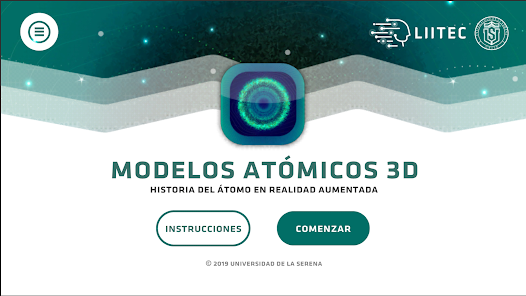
\includegraphics[width =\textwidth]{Imagens/Fig1.png}
\caption{Tela inicial do aplicativo \emph{Modelos Atómicos 3D} (LIITEC-ULS).}
\label{fig-1}
\source{\url{https://play-lh.googleusercontent.com/0uWL-ro1Pqlfs-KLvgMeUeBMYpputC-Due4BQoJK83lS0m9by2lTG_y5vHVAjRvl5W9J=w526-h296-rw}. Acesso em: 6 jun. 2025.}
\end{minipage}
\end{figure}

Os alunos receberam QR Codes que permitiram o acesso aos modelos tridimensionais interativos dos átomos, promovendo uma transição significativa do papel de ouvintes passivos a protagonistas do processo de aprendizagem, interagindo de forma autônoma e colaborativa com os conteúdos.

A análise linguística das transcrições evidenciou mudanças qualitativas no discurso dos estudantes. Durante a atividade com RA, observou-se um aumento expressivo na frequência e na complexidade das interações verbais. Termos como ``núcleo", ``elétron", ``camada eletrônica", ``massa concentrada" e ``energia" passaram a ser utilizados com maior propriedade e contextualização, demonstrando apropriação conceitual e integração da linguagem científica ao vocabulário dos alunos. Essa apropriação linguística, conforme \textcite{vygotsky2000}, é indicativa do avanço no processo de internalização dos conceitos, sendo mediada pelo desenvolvimento das funções mentais superiores por meio da cultura e da interação social proporcionada pela RA. Foi possível registrar algumas interações verbais entre os estudantes:

\begin{quote}
    No quadro eu não entendi direito, mas com o celular ficou bem mais fácil. (E5)
    
Nossa, ele se movimentou exatamente como você falou, professora. (E15)

Tá igual os exemplos do quadro, mas assim é bem mais fácil. (E13)
\end{quote}

Os discursos passaram a refletir maior autorregulação cognitiva, com alunos verbalizando hipóteses, confirmando observações com os colegas e elaborando descrições mais precisas dos modelos atômicos. Também se identificou o uso de linguagem colaborativa, com expressões como ``olha aqui", ``eu acho que esse é o núcleo" ou ``isso aqui parece com o que vimos antes", que indicam construção coletiva do conhecimento e fortalecimento de interações dialógicas.

Essas transformações nos padrões discursivos revelam não apenas o impacto da RA na cognição, mas também sua influência sobre os modos de comunicação e de produção de sentidos no ambiente escolar. Conforme argumentam \textcite{caberoalmenara2025} e \textcite{bacca2014}, experiências de aprendizagem imersiva promovem um ambiente mais propício à expressão verbal significativa, em que os estudantes não apenas repetem conceitos, mas os reelaboram com base na interação ativa com os objetos de estudo.

\subsection{Investigação de como os discursos são produzidos, distribuídos e consumidos no contexto escolar}
A reação dos estudantes ao utilizar a RA foi imediata e expressiva. Essa mudança é amplamente discutida por \textcite{silva2011realidade}, que apontam como a RA favorece a participação ativa, a experimentação e a criatividade dos alunos, além de proporcionar igual oportunidade de comunicação e permitir a repetição de experiências fora do tempo e espaço tradicionais da sala de aula. Alguns relatos dos estudantes:

\begin{quote}
    Isso é impressionante, não sabia que seria tão legal assim! (E11)
    
Assim fica bem fácil identificar cada estrutura, dá pra ver o núcleo, a eletrosfera e os elétrons, exatamente como a professora falou. (E20)
\end{quote}

Relatos espontâneos e gestos corporais revelaram surpresa e entusiasmo ao visualizarem, de forma dinâmica, elementos como a eletrosfera em movimento ao redor do núcleo atômico. Alguns alunos, fascinados com a experiência, chegaram a estender as mãos na tentativa de tocar os objetos virtuais, demonstrando elevado grau de imersão e curiosidade. Esse momento foi caracterizado como especialmente rico do ponto de vista pedagógico, uma vez que a visualização tridimensional proporcionou maior concretude a conceitos tradicionalmente abstratos, facilitando a construção de significados e a internalização dos conteúdos.

O entusiasmo e a imersão relatados pelos estudantes deste estudo, ao tentarem ``tocar" os modelos virtuais ou ao verbalizarem descobertas sobre a estrutura atômica, exemplificam o que \textcite{pereira2017} afirmam sobre a capacidade da RA de atingir áreas da cognição pouco acessíveis por métodos convencionais, especialmente ao tornar visível e manipulável o que é abstrato e invisível na química escolar.

A mudança qualitativa observada com a introdução da RA, marcada pelo entusiasmo, surpresa e apropriação conceitual dos estudantes, encontra respaldo em \textcite{caberoalmenara2025}, que enfatizam como as tecnologias de realidade mista (aumentada e virtual) promovem benefícios cognitivos e cinestésicos, estimulando habilidades visuais, espaciais e reflexivas pouco acessíveis por métodos tradicionais. Esses autores destacam ainda que a manipulação ativa de objetos virtuais favorece o desenvolvimento de competências gráficas e a mobilização de diferentes habilidades cognitivas, ampliando o espectro de aprendizagem.

O relato dos alunos ao tentarem ``tocar" os modelos virtuais ou ao descreverem com precisão estruturas atômicas ilustra o impacto da experiência imersiva na construção do conhecimento, como defendem \textcite{caberoalmenara2025} e \textcite{gleason2020}, ao fundamentarem o valor do aprendizado experiencial e construtivista.

A análise dos dados evidenciou que a inserção da RA não apenas potencializou o interesse e a participação dos alunos, como também promoveu uma mudança qualitativa nos discursos e nas interações em sala de aula. Os estudantes passaram a empregar uma linguagem mais precisa e articulada ao descrever os modelos atômicos, demonstrando maior domínio conceitual e envolvimento com a temática.

Esse fenômeno está alinhado com os achados de \textcite{bacca2014}, \textcite{huang2018}, que identificaram na literatura que a RA não só facilita a compreensão de conteúdos complexos, mas também promove colaboração, interação e motivação intrínseca, renovando o interesse dos estudantes pelas disciplinas científicas.

Essas pesquisas reforçam o potencial das tecnologias imersivas como ferramentas mediadoras da aprendizagem, especialmente no ensino de Ciências, ao proporcionarem experiências significativas que favorecem o engajamento cognitivo e a motivação intrínseca dos estudantes.

Segundo \textcite{santos2023}, \textcite{tito2022}, a RA pode transformar aulas tradicionalmente desafiadoras em experiências mais participativas e significativas, como mostram estudos de oficinas e intervenções com aplicativos de RA em química e biologia. Esses autores relatam ganhos em engajamento, retenção de conteúdo e desenvolvimento de habilidades cognitivas e digitais, confirmando que a visualização tridimensional de estruturas atômicas facilita o entendimento espacial e a internalização dos conceitos, como observado neste estudo.

Na \Cref{fig-2}, por exemplo, apresenta o modelo atômico proposto por Thomson, físico britânico vencedor do Nobel de Física, creditado com a descoberta e identificação do elétron, a primeira partícula subatômica a ser descrita \cite{oliveira2021}.

%--- CÓDIGO DA FIGURA 2 ---%
\begin{figure}[htbp]
\centering
\begin{minipage}{0.65\textwidth}
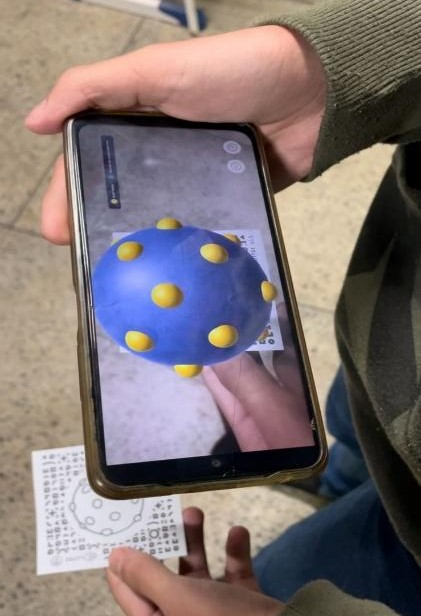
\includegraphics[angle=90,width =\textwidth]{Imagens/Fig2.jpg}
\caption{Modelo atômico de Thomson.}
\label{fig-2}
\source{Arquivo das autoras (2025).}
\end{minipage}
\end{figure}

Observou-se interesse despertado a partir da visualização da estrutura esférica com elétrons distribuídos uniformemente. Expressões como ``parece que os elétrons estão flutuando" revelam o impacto da tecnologia na representação concreta de conceitos abstratos. A visualização tridimensional da estrutura esférica com elétrons distribuídos uniformemente despertou interesse e curiosidade, evidenciada por expressões como ``parece que os elétrons estão flutuando". Esse tipo de reação revela o impacto da tecnologia na representação concreta de conceitos abstratos, facilitando a compreensão do modelo atômico de Thomson.

O modelo de Thomson, descreve o átomo como uma esfera de carga positiva na qual elétrons (partículas negativas) estão distribuídos de forma uniforme, semelhante a passas em um pudim. Essa representação, tradicionalmente difícil de visualizar, ganhou maior tangibilidade com o uso da realidade aumentada, que permitiu aos estudantes observarem dinamicamente a disposição dos elétrons e a neutralidade da carga atômica.

Deste aspecto, observou-se uma reconfiguração no papel do professor, que passou a atuar como mediador do processo discursivo, incentivando a reflexão crítica e a articulação entre os conhecimentos experienciados e os conteúdos curriculares. A inserção da RA promoveu a emergência de novos gêneros discursivos, como a descrição multimodal e a narrativa de descoberta, mobilizando práticas de letramento científico relevantes para o desenvolvimento da linguagem técnica.

Os discursos gerados em sala se estenderam para outros espaços sociais, com alunos relatando suas experiências para familiares e colegas, o que demonstra a circulação ampliada e o potencial formativo da RA também fora do ambiente escolar. Assim, os discursos escolares tornam-se mais significativos ao dialogarem com práticas culturais contemporâneas e ao se conectarem com o cotidiano dos estudantes.

\subsection{Relação entre os discursos e estruturas de poder/influência na sala de aula}
A interação com o modelo virtual estimulou manifestações espontâneas e gestos corporais que indicam imersão e envolvimento, como tentativas de ``tocar" os elétrons virtuais, reforçando a capacidade da RA em promover uma aprendizagem mais ativa e sensorial.

A reação dos alunos corrobora a importância de tornar o saber científico acessível e significativo no ensino, pois o engajamento e a motivação autônoma dos estudantes dependem da satisfação de necessidades psicológicas básicas como autonomia, competência e pertencimento \cite{deci2008}. Para que os alunos se envolvam de forma autônoma e desenvolvam motivação intrínseca, é fundamental que o conhecimento seja apresentado de maneira compreensível, relevante e conectada à realidade dos estudantes, permitindo escolhas, participação ativa e sentido pessoal nas atividades propostas.

Assim, conforme \textcite{deci2008}, adaptar o saber científico para formas acessíveis e significativas no ensino é condição essencial para promover a autodeterminação, o interesse genuíno e a aprendizagem de qualidade. A tecnologia, ao proporcionar uma experiência visual e interativa, atua como mediadora dessa transposição, facilitando a internalização dos conceitos atômicos que, de outra forma, permanecem abstratos e distantes da experiência cotidiana dos estudantes.

Dessa forma, a situação observada reflete não apenas o interesse despertado pelo modelo de Thomson em si, mas também a eficácia da realidade aumentada como recurso pedagógico para transformar a abstração científica em conhecimento vivenciado e compreendido pelos alunos.

A atividade permitiu, aos alunos, interagirem com o modelo atômico de Rutherford, observando a concentração de massa no núcleo e o espaço predominantemente vazio ao redor (Figuras \ref{fig-3} e \ref{fig-4}). As falas espontâneas, como ``eu não sabia que tinha tanto espaço vazio no átomo", indicam o favorecimento da compreensão conceitual a partir da mediação tecnológica, evidenciando o potencial da RA como ferramenta didática.

Essas interações revelam também uma reconfiguração das estruturas tradicionais de poder na sala de aula. Com a mediação tecnológica, a centralidade do saber desloca-se do professor para um ambiente mais dialógico e colaborativo, no qual os estudantes assumem maior protagonismo e autonomia no processo de aprendizagem. O docente, por sua vez, atua como mediador das interações e facilitador das descobertas, promovendo uma maior horizontalização das relações pedagógicas e tornando o espaço escolar mais aberto à escuta e à expressão discente.

Além disso, a mediação docente e a utilização da RA favorecem práticas mais inclusivas ao contemplar diferentes estilos de aprendizagem, democratizando o acesso ao conhecimento e ampliando as possibilidades de participação mesmo em contextos marcados por desigualdades educacionais. A experiência imersiva também permitiu uma ressignificação da autoridade do conhecimento científico, que deixou de ser apenas transmitido para ser reconstruído pelos próprios alunos a partir de vivências sensoriais e cognitivas. Relatos como ``dá pra ver o elétron se movimentando em volta do núcleo!" ilustram essa apropriação ativa dos conceitos, reforçando a importância de metodologias que conectem teoria e experiência.

\textcite{santos2023}, \textcite{tito2022} demonstram que a RA e RV favorecem o protagonismo discente, a visualização de conceitos abstratos e a aprendizagem colaborativa, aspectos também identificados neste estudo. \textcite{freitas2022} amplia essa discussão ao mostrar, em sua análise sobre vídeos 360° e realidade virtual, que experiências imersivas estimulam não apenas a cognição, mas também afetos, interesse situacional e competências da cibercultura, promovendo uma aprendizagem mais conectada ao mundo contemporâneo.

Esses achados dialogam com \textcite{nascimento2024}, que ressaltam a importância das metodologias ativas mediadas por tecnologias digitais para o desenvolvimento de competências críticas e adaptativas, especialmente em contextos pós-pandêmicos, nos quais a integração entre tecnologia e prática pedagógica tornou-se ainda mais urgente.

O uso de dispositivos móveis como mediadores da aprendizagem, central neste estudo, também é amplamente discutido por \textcite{nascimento2016, nascimento2017}, que, em revisões sistemáticas, apontam tanto o potencial quanto a carência de pesquisas sobre estratégias pedagógicas inovadoras com tecnologias móveis no Ensino Fundamental.

Em caso análogo, ao estudarem o modelo atômico de Rutherford, físico e químico conhecido como o pai da física nuclear, por meio do aplicativo (\Cref{fig-3}), os alunos puderam visualizar de forma interativa e tridimensional a estrutura nuclear, compreendendo o núcleo compacto contendo prótons e nêutrons, bem como os elétrons orbitando em torno desse núcleo em uma eletrosfera predominantemente vazia. Essa experiência proporcionou uma percepção clara dos espaços vazios no átomo, evidenciada pelas falas dos estudantes, como ``eu não sabia que tinha tanto espaço vazio no átomo", que indicam a apropriação do conceito de que o átomo é formado majoritariamente por espaço vazio, um aspecto fundamental do modelo de Rutherford.

%--- CÓDIGO DA FIGURA 3 ---%
\begin{figure}[htbp]
\centering
\begin{minipage}{0.55\textwidth}
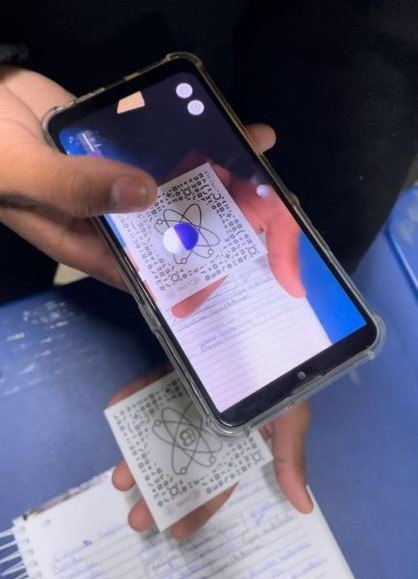
\includegraphics[angle=90,width =\textwidth]{Imagens/Fig3.jpg}
\caption{Modelo atômico de Rutherford.}
\label{fig-3}
\source{Arquivo das autoras (2025).}
\end{minipage}
\end{figure}

%--- CÓDIGO DA FIGURA 4 ---%
\begin{figure}[htbp]
\centering
\begin{minipage}{0.55\textwidth}
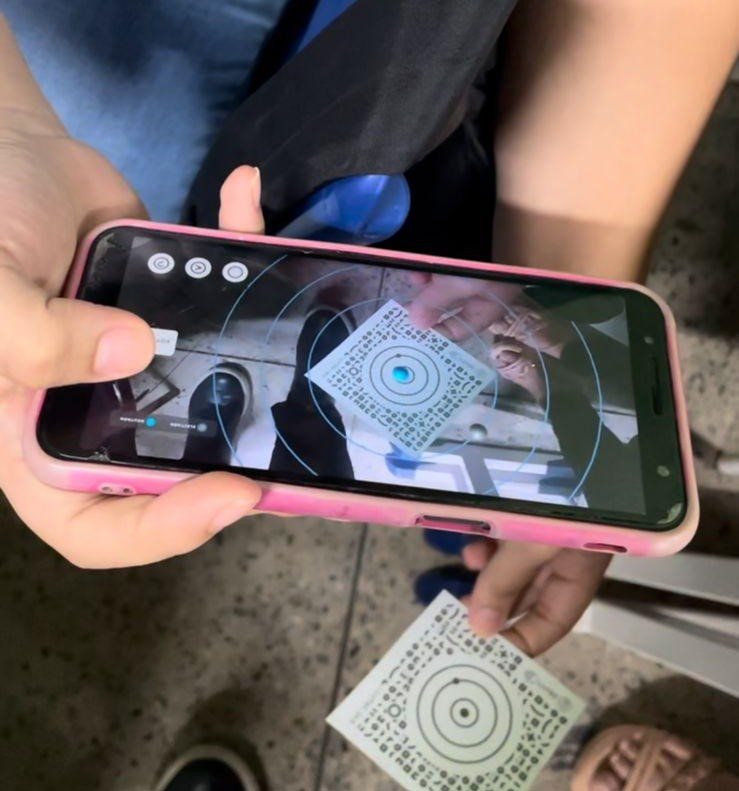
\includegraphics[width =\textwidth]{Imagens/Fig4.jpg}
\caption{Modelo atômico de Bohr.}
\label{fig-4}
\source{Arquivo das autoras (2025).}
\end{minipage}
\end{figure}

A experiência relatada aqui contribui para preencher uma lacuna, ao evidenciar que a RA pode transformar a relação dos alunos com conteúdos tradicionalmente abstratos, promovendo maior engajamento, participação e domínio conceitual. Ao inserir elementos da cultura digital juvenil no cotidiano escolar, fortalece-se o agenciamento estudantil e estreitam-se os vínculos entre o currículo e as vivências contemporâneas dos estudantes. Para \textcite{vygotsky2000}, a participação ativa do aluno, mediada pela colaboração e pelo diálogo, potencializa o desenvolvimento cognitivo, permitindo que o estudante avance além do que conseguiria sozinho.

Os estudantes também interagiram com o modelo atômico de Bohr, físico que fez contribuições essenciais para a compreensão da estrutura atômica e da mecânica quântica, visualizando camadas eletrônicas ao redor do núcleo, com ênfase nos níveis de energia propostos pelo cientista (\Cref{fig-4}). A percepção do movimento e da estrutura concentrou a atenção dos alunos, sendo registrada a fala: ``dá pra ver o elétron se movimentando em volta do núcleo!", o que demonstra a apropriação dos conceitos científicos por meio de visualização dinâmica.

As interações dos estudantes após o uso da RA revelam uma apropriação mais articulada da linguagem científica e uma postura mais investigativa, aspectos que, segundo \textcite{caberoalmenara2025}, são fundamentais para a aprendizagem experiencial e reflexiva. A integração da RA ao ensino de ciências, portanto, não apenas potencializa o interesse e a compreensão conceitual, mas também favorece a construção de um ambiente de aprendizagem mais dinâmico e colaborativo. Esses resultados reforçam a necessidade de investir em formação docente, infraestrutura tecnológica e metodologias ativas, para que o potencial transformador das tecnologias imersivas seja plenamente realizado no contexto da educação básica.

É importante destacar que, apesar dos desafios técnicos e da necessidade de formação docente, a literatura aponta que a integração efetiva da RA ao currículo pode promover uma aprendizagem mais ativa, colaborativa e contextualizada, alinhada às expectativas dos estudantes do século XXI. \textcite{nascimento2016, nascimento2017}, apontam tanto o potencial quanto a carência de pesquisas sobre estratégias pedagógicas inovadoras com tecnologias móveis no Ensino Fundamental. A experiência contribui para preencher uma lacuna: oferecer experiências de aprendizado imersivas e interativas, permitindo que os alunos explorem ambientes inacessíveis, visualizem conceitos complexos em 3D e pratiquem habilidades em cenários seguros. Ao evidenciar que a RA pode transformar a relação dos alunos com conteúdos tradicionalmente abstratos, o docente promove maior engajamento, participação e domínio conceitual em suas aulas.

Assim, esses resultados não apenas confirmam, mas também expandem a compreensão sobre o potencial da RA como ferramenta mediadora da aprendizagem em ciências, especialmente ao evidenciar sua capacidade de transformar o engajamento e a motivação dos alunos diante de conteúdos tradicionalmente abstratos e desafiadores.

\section{Conclusão}
Este estudo teve como objetivo identificar os impactos da realidade aumentada (RA) no engajamento e motivação de estudantes do 9º ano do Ensino Fundamental durante o aprendizado dos modelos atômicos. A pesquisa em tela evidenciou que a integração da RA, por meio do aplicativo \emph{Modelos Atómicos 3D}, promoveu uma transformação significativa no processo de aprendizagem, ao estimular maior participação ativa, interesse e compreensão conceitual dos alunos.

A adoção de uma metodologia interativa e imersiva, em substituição à abordagem expositiva tradicional centrada no professor e em recursos visuais estáticos, revelou-se eficaz para criar um ambiente de aprendizagem mais dinâmico, participativo e centrado no estudante.

O uso do aplicativo \emph{Modelos Atómicos 3D} possibilitou aos alunos a vivência concreta de conceitos abstratos, como a movimentação de partículas subatômicas e a estrutura dos diferentes modelos atômicos, facilitando a assimilação dos conteúdos e despertando a curiosidade e o interesse pela ciência. A visualização tridimensional e interativa desses elementos facilitou a assimilação dos conteúdos, ao mesmo tempo em que despertou a curiosidade e ampliou o interesse pela temática científica.

Observou-se uma mudança significativa no comportamento dos estudantes, que passaram de uma postura passiva e dispersa para uma atuação ativa, curiosa e colaborativa, evidenciando o potencial das tecnologias imersivas para promover motivação autônoma e engajamento. A motivação autônoma, caracterizada pela realização das atividades por interesse próprio, liberdade de escolha e alinhamento com valores pessoais, demonstrou-se fundamental para o envolvimento dos alunos, favorecendo o esforço, a persistência e a participação entusiástica nas tarefas propostas. Essa qualidade motivacional, além de potencializar o aprendizado, contribui para a formação de estudantes mais autônomos, críticos e protagonistas do próprio processo educativo.

Os relatos espontâneos e as reações físicas de encantamento e envolvimento dos alunos indicam que a RA não apenas contribui para tornar o conteúdo mais acessível, mas também favorece o protagonismo discente, permitindo que os estudantes se apropriem do processo de aprendizagem de maneira mais significativa.

Conclui-se que o uso da RA no ensino de modelos atômicos não apenas enriquece o processo de ensino e aprendizagem, mas também se configura como uma estratégia pedagógica potente para fomentar o interesse pela ciência, aumentar a motivação intrínseca dos estudantes e estimular práticas pedagógicas mais inovadoras e inclusivas. Sugere-se, portanto, a ampliação do uso de recursos de RA em diferentes componentes curriculares, bem como a realização de formações continuadas para professores, visando explorar de forma mais ampla e qualificada o potencial transformador dessas tecnologias no contexto educacional.


\printbibliography\label{sec-bib}
% if the text is not in Portuguese, it might be necessary to use the code below instead to print the correct ABNT abbreviations [s.n.], [s.l.]
%\begin{portuguese}
%\printbibliography[title={Bibliography}]
%\end{portuguese}


%full list: conceptualization,datacuration,formalanalysis,funding,investigation,methodology,projadm,resources,software,supervision,validation,visualization,writing,review
\begin{contributors}[sec-contributors]
\authorcontribution{Karla Angélica Silva do Nascimento}[formalanalysis,validation,supervision,methodology,writing,review]
\authorcontribution{Viviane dos Santos Marques}[conceptualization,methodology,datacuration,writing,review]
\end{contributors}


\end{document}

